% questions.tex —— 2010 年·普通高等学校招生考试·安徽卷·理科 · 题目内容片段（无答案）
% 由 tools/generate_projects.py 依来源总账自 2010/2010_数学真题_安徽理_试题.md 生成，勿手改（改源 MD 后重跑）


状态：needs-review；依固定候选 PDF 两页（印刷页 569–570）逐题核验，五幅图已矢量重绘。原页未印分值，不补。

\gkpart{一、选择题}

\begin{question}
\gkti{1}$\mathrm i$ 是虚数单位，$\dfrac{\mathrm i}{\sqrt3+3\mathrm i}=$（　）

（A）$\dfrac14-\dfrac{\sqrt3}{12}\mathrm i$

（B）$\dfrac14+\dfrac{\sqrt3}{12}\mathrm i$

（C）$\dfrac12+\dfrac{\sqrt3}{6}\mathrm i$

（D）$\dfrac12-\dfrac{\sqrt3}{6}\mathrm i$

\end{question}
\begin{question}
\gkti{2}若集合 $A=\left\{x\middle|\log_{\frac12}x\geqslant\dfrac12\right\}$，则 $\complement_{\mathbf R}A=$（　）

（A）$(-\infty,0]\cup\left(\dfrac{\sqrt2}2,+\infty\right)$

（B）$\left(\dfrac{\sqrt2}2,+\infty\right)$

（C）$(-\infty,0]\cup\left[\dfrac{\sqrt2}2,+\infty\right)$

（D）$\left[\dfrac{\sqrt2}2,+\infty\right)$

\end{question}
\begin{question}
\gkti{3}设向量 $\boldsymbol a=(1,0)$，$\boldsymbol b=\left(\dfrac12,\dfrac12\right)$，则下列结论中正确的是（　）

（A）$|\boldsymbol a|=|\boldsymbol b|$

（B）$\boldsymbol a\cdot\boldsymbol b=\dfrac{\sqrt2}2$

（C）$\boldsymbol a-\boldsymbol b$ 与 $\boldsymbol b$ 垂直

（D）$\boldsymbol a\parallel\boldsymbol b$

\end{question}
\begin{question}
\gkti{4}若 $f(x)$ 是 $\mathbf R$ 上周期为 $5$ 的奇函数，且满足 $f(1)=1$，$f(2)=2$，则 $f(3)-f(4)=$（　）

（A）$-1$

（B）$1$

（C）$-2$

（D）$2$

\end{question}
\begin{question}
\gkti{5}双曲线方程为 $x^2-2y^2=1$，则它的右焦点坐标为（　）

（A）$\left(\dfrac{\sqrt2}2,0\right)$

（B）$\left(\dfrac{\sqrt5}2,0\right)$

（C）$\left(\dfrac{\sqrt6}2,0\right)$

（D）$(\sqrt3,0)$

\Needspace{0.4\textheight}
\end{question}
\begingroup
\renewenvironment{question}{\Needspace{0.5\textheight}}{}
\begin{question}
\gkti{6}设 $abc>0$，二次函数 $f(x)=ax^2+bx+c$ 的图象可能是（　）
\nopagebreak[4]
\begin{center}% 2010 年安徽卷理科第 6 题：四个二次函数图象选项（A）—（D）。
% 来源 PDF：普通高考/2010/2010安徽理.pdf，SHA-256 2760eb9e09374139a51303b0c2590746c74dfef7fed99ac6b2eace305af646c5。
% 原页：第 1 页（A3 三栏）第 1 栏，书页码 569。
% 重绘依据：四幅均只示意开口方向、y 轴截距符号与对称轴位置，不标刻度：
%   (A) 开口向下、截距为负、顶点在 y 轴左侧；(B) 开口向下、截距为正、顶点在右侧；
%   (C) 开口向上、截距为正、顶点在右侧；(D) 开口向上、截距为负、顶点在右侧。
\begin{tikzpicture}[semithick, scale=1.15, every node/.style={inner sep=1.2pt, font=\small}]
  % (A)
  \begin{scope}[shift={(0,0)}]
    \draw[-stealth] (-1.75,0) -- (0.75,0) node[right] {$x$};
    \draw[-stealth] (0,-0.95) -- (0,0.65) node[above] {$y$};
    \draw[thick,domain=-1.55:0.10,samples=80] plot (\x,{-0.8*(\x+0.9)^2+0.3});
    \node[below] at (-0.45,-1.35) {（A）};
  \end{scope}
  % (B)
  \begin{scope}[shift={(3.3,0)}]
    \draw[-stealth] (-0.55,0) -- (1.95,0) node[right] {$x$};
    \draw[-stealth] (0,-0.65) -- (0,1.05) node[above] {$y$};
    \draw[thick,domain=-0.45:1.85,samples=80] plot (\x,{-0.8*(\x-0.7)^2+0.9});
    \node[below] at (0.7,-1.35) {（B）};
  \end{scope}
  % (C)
  \begin{scope}[shift={(0,-3.1)}]
    \draw[-stealth] (-1.65,0) -- (1.65,0) node[right] {$x$};
    \draw[-stealth] (0,-0.75) -- (0,0.85) node[above] {$y$};
    \draw[thick,domain=-0.20:1.60,samples=80] plot (\x,{0.8*(\x-0.7)^2-0.2});
    \node[below] at (0.45,-1.35) {（C）};
  \end{scope}
  % (D)
  \begin{scope}[shift={(3.3,-3.1)}]
    \draw[-stealth] (-0.40,0) -- (1.95,0) node[right] {$x$};
    \draw[-stealth] (0,-0.80) -- (0,0.75) node[above] {$y$};
    \draw[thick,domain=-0.25:1.80,samples=80] plot (\x,{0.8*(\x-0.75)^2-0.6});
    \node[below] at (0.75,-1.35) {（D）};
  \end{scope}
\end{tikzpicture}
\end{center}
\nopagebreak[4]
\end{question}
\endgroup
\begin{question}
\gkti{7}设曲线 $C$ 的参数方程为 $\begin{cases}x=2+3\cos\theta,\\ y=-1+3\sin\theta\end{cases}$（$\theta$ 为参数），直线 $l$ 的方程为 $x-3y+2=0$，则曲线 $C$ 上到直线 $l$ 的距离为 $\dfrac{7\sqrt{10}}{10}$ 的点的个数为（　）

（A）$1$

（B）$2$

（C）$3$

（D）$4$

\Needspace{0.4\textheight}
\end{question}
\begingroup
\renewenvironment{question}{\Needspace{0.5\textheight}}{}
\begin{question}
\gkti{8}一个几何体的三视图如图，该几何体的表面积为（　）
\nopagebreak[4]
\begin{center}% 2010 年安徽卷理科第 8 题：几何体的三视图（正视图、侧视图、俯视图）。
% 来源 PDF：普通高考/2010/2010安徽理.pdf，SHA-256 2760eb9e09374139a51303b0c2590746c74dfef7fed99ac6b2eace305af646c5。
% 原页：第 1 页（A3 三栏）第 2 栏上部，书页码 569。
% 重绘依据：下部长方体 8×10×2；上部长方体 6×2×8，居中置于下部之上。
% 正视图宽 8、高 2，上部宽 6、两侧各 1；侧视图深 10、高 2，上部深 2、偏右 2；
% 俯视图 8×10，内框 6×2、距下边 2。
\begin{tikzpicture}[semithick, scale=0.38, every node/.style={inner sep=1.5pt, font=\small}]
  % 正视图
  \draw (0,0) rectangle (8,2);
  \draw (1,2) rectangle (7,10);
  \draw[<->] (0,10.45) -- node[above] {$1$} (1,10.45);
  \draw[<->] (1,10.45) -- node[above] {$6$} (7,10.45);
  \draw[<->] (7,10.45) -- node[above] {$1$} (8,10.45);
  \draw[<->] (-0.45,0) -- node[left] {$2$} (-0.45,2);
  \draw[<->] (-0.45,2) -- node[left] {$8$} (-0.45,10);

  % 侧视图
  \draw (11,0) rectangle (21,2);
  \draw (17,2) rectangle (19,10);
  \draw[<->] (11,10.45) -- node[above] {$6$} (17,10.45);
  \draw[<->] (17,10.45) -- node[above] {$2$} (19,10.45);
  \draw[<->] (19,10.45) -- node[above] {$2$} (21,10.45);
  \draw[<->] (21.45,0) -- node[right] {$2$} (21.45,2);
  \draw[<->] (21.45,2) -- node[right] {$8$} (21.45,10);

  % 俯视图
  \draw (4,-14) rectangle (12,-4);
  \draw (5,-12) rectangle (11,-10);
  \draw[<->] (12.45,-4) -- node[right] {$6$} (12.45,-10);
  \draw[<->] (12.45,-10) -- node[right] {$2$} (12.45,-12);
  \draw[<->] (12.45,-12) -- node[right] {$2$} (12.45,-14);
  \draw[<->] (4,-14.45) -- node[below] {$8$} (12,-14.45);

  \node at (4,-2.25) {正（主）视图};
  \node at (16,-2.25) {侧（左）视图};
  \node at (8,-16.2) {俯视图};
\end{tikzpicture}
\end{center}
\nopagebreak[4]
（A）$280$

（B）$292$

（C）$360$

（D）$372$

\end{question}
\endgroup
\begin{question}
\gkti{9}动点 $A(x,y)$ 在圆 $x^2+y^2=1$ 上绕坐标原点沿逆时针方向匀速旋转，$12$ 秒旋转一周。已知时间 $t=0$ 时，点 $A$ 的坐标是 $\left(\dfrac12,\dfrac{\sqrt3}2\right)$，则当 $0\leqslant t\leqslant12$ 时，动点 $A$ 的纵坐标 $y$ 关于 $t$（单位：秒）的函数的单调递增区间是（　）

（A）$[0,1]$

（B）$[1,7]$

（C）$[7,12]$

（D）$[0,1]$ 和 $[7,12]$

\end{question}
\begin{question}
\gkti{10}设 $\{a_n\}$ 是任意等比数列，它的前 $n$ 项和，前 $2n$ 项和与前 $3n$ 项和分别为 $X$，$Y$，$Z$，则下列等式中恒成立的是（　）

（A）$X+Z=2Y$

（B）$Y(Y-X)=Z(Z-X)$

（C）$Y^2=XZ$

（D）$Y(Y-X)=X(Z-X)$

\end{question}
\gkpart{二、填空题}

\begin{question}
\gkti{11}命题“对任何 $x\in\mathbf R$，$|x-2|+|x-4|>3$”的否定是$\underline{\qquad}$。

\end{question}
\begin{question}
\gkti{12}$\left(\dfrac{x}{\sqrt y}-\dfrac{y}{\sqrt x}\right)^6$ 的展开式中，$x^3$ 的系数等于$\underline{\qquad}$。

\end{question}
\begin{question}
\gkti{13}设 $x$，$y$ 满足约束条件 $\begin{cases}2x-y+2\geqslant0,\\ 8x-y-4\leqslant0,\\ x\geqslant0,\ y\geqslant0,\end{cases}$ 若目标函数 $z=abx+y$（$a>0$，$b>0$）的最大值为 $8$，则 $a+b$ 的最小值为$\underline{\qquad}$。

\Needspace{0.4\textheight}
\end{question}
\begingroup
\renewenvironment{question}{\Needspace{0.5\textheight}}{}
\begin{question}
\gkti{14}如图所示，程序框图（算法流程图）的输出值 $x=$ $\underline{\qquad}$。
\nopagebreak[4]
\begin{center}% 2010 年安徽卷理科第 14 题：算法流程图。
% 来源 PDF：普通高考/2010/2010安徽理.pdf，SHA-256 2760eb9e09374139a51303b0c2590746c74dfef7fed99ac6b2eace305af646c5。
% 原页：第 1 页（A3 三栏）第 3 栏上部，书页码 569。
% 重绘依据：开始 → x=1 → 判断「x 是奇数?」；是（右）→ x=x+1 → 回到判断前；
%   否（下）→ x=x+2 → 判断「x>8?」；否（右）→ 回到「x 是奇数?」前；是（下）→ 输出 x → 结束。
\begin{tikzpicture}[semithick, >=Stealth,
  every node/.style={inner sep=1.5pt, font=\small}]
  \node (start) [draw, rounded corners=4pt, minimum width=1.9cm, minimum height=0.55cm] at (0,0) {开始};
  \node (x1) [draw, minimum width=1.9cm, minimum height=0.55cm] at (0,-1.35) {$x=1$};
  \node (c1) [draw, diamond, aspect=2.1, minimum width=3.1cm,
    minimum height=1.15cm] at (0,-3.15) {$x$ 是奇数?};
  \node (p1) [draw, minimum width=2.5cm, minimum height=0.55cm] at (3.7,-3.15) {$x=x+1$};
  \node (p2) [draw, minimum width=2.5cm, minimum height=0.55cm] at (0,-4.85) {$x=x+2$};
  \node (c2) [draw, diamond, aspect=2.1, minimum width=3.1cm,
    minimum height=1.15cm] at (0,-6.65) {$x>8?$};
  \node (out) [draw, trapezium, trapezium left angle=72, trapezium right angle=108,
    minimum width=2.4cm, minimum height=0.55cm] at (0,-8.25) {输出 $x$};
  \node (end) [draw, rounded corners=4pt, minimum width=1.9cm, minimum height=0.55cm] at (0,-9.45) {结束};

  \draw[->] (start) -- (x1);
  \draw[->] (x1) -- (c1);
  \draw[->] (c1.east) -- node[above] {是} (p1.west);
  \draw[->] (c1.south) -- node[right] {否} (p2.north);
  \draw[->] (p2) -- (c2);
  \draw[->] (c2.south) -- node[right] {是} (out.north);
  \draw[->] (out) -- (end);
  % x=x+1 的回流
  \draw (p1.north) -- (3.7,-2.0) -- (0,-2.0);
  % x>8? 为否时的回流
  \draw (c2.east) -- node[above] {否} (5.2,-6.65) -- (5.2,-2.0) -- (0,-2.0);
  \draw[->] (0,-2.0) -- (c1.north);
\end{tikzpicture}
\end{center}
\nopagebreak[4]
\end{question}
\endgroup
\begin{question}
\gkti{15}甲罐中有 $5$ 个红球，$2$ 个白球和 $3$ 个黑球，乙罐中有 $4$ 个红球，$3$ 个白球和 $3$ 个黑球，先从甲罐中随机取出一球放入乙罐，分别以 $A_1$，$A_2$ 和 $A_3$ 表示由甲罐取出的球是红球，白球和黑球的事件；再从乙罐中随机取出一球，以 $B$ 表示由乙罐取出的球是红球的事件，则下列结论中正确的是$\underline{\qquad}$。（写出所有正确结论的编号）

① $P(B)=\dfrac25$；

② $P(B\mid A_1)=\dfrac5{11}$；

③ 事件 $B$ 与事件 $A_1$ 相互独立；

④ $A_1$，$A_2$，$A_3$ 是两两互斥的事件；

⑤ $P(B)$ 的值不能确定，因为它与 $A_1$，$A_2$，$A_3$ 中究竟哪一个发生有关。

\end{question}
\gkpart{三、解答题}

\begin{question}
\gkti{16}设 $\triangle ABC$ 是锐角三角形，$a$，$b$，$c$ 分别是内角 $A$、$B$、$C$ 所对边长，并且

\nopagebreak[4]
\[\sin^2A=\sin\left(\frac\pi3+B\right)\sin\left(\frac\pi3-B\right)+\sin^2B.\]

（1）求角 $A$ 的值；

（2）若 $\overrightarrow{AB}\cdot\overrightarrow{AC}=12$，$a=2\sqrt7$，求 $b$，$c$（其中 $b<c$）。

\end{question}
\begin{question}
\gkti{17}设 $a$ 为实数，函数 $f(x)=\mathrm e^x-2x+2a$，$x\in\mathbf R$。

（1）求 $f(x)$ 的单调区间与极值；

（2）求证：当 $a>\ln2-1$ 且 $x>0$ 时，$\mathrm e^x>x^2-2ax+1$。

\Needspace{0.4\textheight}
\end{question}
\begingroup
\renewenvironment{question}{\Needspace{0.5\textheight}}{}
\begin{question}
\gkti{18}如图，在多面体 $ABCDEF$ 中，四边形 $ABCD$ 是正方形，$EF\parallel AB$，$EF\perp FB$，$AB=2EF$，$\angle BFC=90^\circ$，$BF=FC$，$H$ 为 $BC$ 的中点。

（1）求证：$FH\parallel$ 平面 $EDB$；

（2）求证：$AC\perp$ 平面 $EDB$；

（3）求二面角 $B-DE-C$ 的大小。
\nopagebreak[4]
\begin{center}% 2010 年安徽卷理科第 18 题：多面体 ABCDEF。
% 来源 PDF：普通高考/2010/2010安徽理.pdf，SHA-256 2760eb9e09374139a51303b0c2590746c74dfef7fed99ac6b2eace305af646c5。
% 原页：第 2 页（A3 三栏）第 1 栏下部，书页码 570。
% 重绘依据：ABCD 为正方形，EF∥AB 且 EF=AB/2；F 在 C 上方、E 在 D 上方；
%   BF、CF、EF、ED、EA、AB、BC、AD 为实线；CD、AC、BD 为不可见棱，画虚线；H 为 BC 中点。
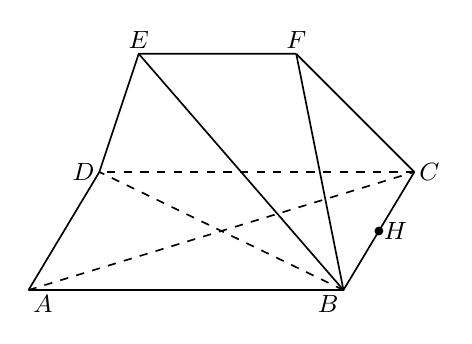
\begin{tikzpicture}[semithick, every node/.style={inner sep=1.5pt, font=\small}]
  \coordinate (A) at (0,0);
  \coordinate (B) at (4,0);
  \coordinate (C) at (4.9,1.5);
  \coordinate (D) at (0.9,1.5);
  \coordinate (E) at (1.4,3.0);
  \coordinate (F) at (3.4,3.0);
  \coordinate (H) at (4.45,0.75);

  \draw (A) -- (B) -- (C);
  \draw (A) -- (D) -- (E) -- (F) -- (E);
  \draw (F) -- (C);
  \draw (F) -- (B);
  \draw (E) -- (B);
  \draw[dashed] (C) -- (D);
  \draw[dashed] (A) -- (C);
  \draw[dashed] (B) -- (D);

  \fill (H) circle (1.6pt);
  \node[below right] at (A) {$A$};
  \node[below left] at (B) {$B$};
  \node[right] at (C) {$C$};
  \node[left] at (D) {$D$};
  \node[above] at (E) {$E$};
  \node[above] at (F) {$F$};
  \node[right] at (H) {$H$};
\end{tikzpicture}
\end{center}
\nopagebreak[4]
\Needspace{0.4\textheight}
\end{question}
\endgroup
\begingroup
\renewenvironment{question}{\Needspace{0.5\textheight}}{}
\begin{question}
\gkti{19}如图，已知椭圆 $E$ 经过点 $A(2,3)$，对称轴为坐标轴，焦点 $F_1$，$F_2$ 在 $x$ 轴上，离心率 $e=\dfrac12$。

（1）求椭圆 $E$ 的方程；

（2）求 $\angle F_1AF_2$ 的角平分线所在直线 $l$ 的方程；

（3）在椭圆 $E$ 上是否存在关于直线 $l$ 对称的相异两点？若存在，请找出；若不存在，说明理由。
\nopagebreak[4]
\begin{center}% 2010 年安徽卷理科第 19 题：椭圆 E、焦点 F1、F2、点 A 与角平分线 l。
% 来源 PDF：普通高考/2010/2010安徽理.pdf，SHA-256 2760eb9e09374139a51303b0c2590746c74dfef7fed99ac6b2eace305af646c5。
% 原页：第 2 页（A3 三栏）第 2 栏中部，书页码 570。
% 重绘依据：椭圆 x^2/16+y^2/12=1，F1(-2,0)、F2(2,0)，A(2,3)；
%   l 为 ∠F1AF2 的角平分线，方程 2x-y-1=0。
\begin{tikzpicture}[semithick, scale=0.95, every node/.style={inner sep=1.6pt, font=\small}]
  \draw[-stealth] (-4.6,0) -- (4.6,0) node[right] {$x$};
  \draw[-stealth] (0,-3.9) -- (0,4.1) node[above] {$y$};
  \draw[thick] (0,0) ellipse (4 and 3.464);
  \fill (-2,0) circle (1.6pt) node[below] {$F_1$};
  \fill (2,0) circle (1.6pt) node[below] {$F_2$};
  \fill (2,3) circle (1.6pt) node[above right] {$A$};
  \node[below left] at (0,0) {$O$};
  \draw[thick] (-0.25,-1.5) -- (2.15,3.3);
  \node[left] at (-0.25,-1.5) {$l$};
\end{tikzpicture}
\end{center}
\nopagebreak[4]
\end{question}
\endgroup
\begin{question}
\gkti{20}设数列 $a_1$，$a_2$，$\cdots$，$a_n$，$\cdots$ 中的每一项都不为 $0$。证明：$\{a_n\}$ 为等差数列的充分必要条件是：对任何 $n\in\mathbf N_+$，都有

\nopagebreak[4]
\[\frac1{a_1a_2}+\frac1{a_2a_3}+\cdots+\frac1{a_na_{n+1}}=\frac{n}{a_1a_{n+1}}.\]

\end{question}
\begin{question}
\gkti{21}品酒师需定期接受酒味鉴别功能测试，一般通常采用的测试方法如下：拿出 $n$ 瓶外观相同但品质不同的酒让其品尝，要求其按品质优劣为它们排序；经过一段时间，等其记忆淡忘之后，再让其品尝这 $n$ 瓶酒，并重新按品质优劣为它们排序，这称为一轮测试。根据一轮测试中的两次排序的偏离程度的高低为其评分。

现设 $n=4$，分别以 $a_1$，$a_2$，$a_3$，$a_4$ 表示第一次排序时被排为 $1,2,3,4$ 的四种酒在第二次排序时的序号，并令 $X=|1-a_1|+|2-a_2|+|3-a_3|+|4-a_4|$，则 $X$ 是对两次排序的偏离程度的一种描述。

（1）写出 $X$ 的可能值集合；

（2）假设 $a_1$，$a_2$，$a_3$，$a_4$ 等可能的为 $1,2,3,4$ 的各种排列，求 $X$ 的分布列；

（3）某品酒师在相继进行的三轮测试中，都有 $X\leqslant2$，

① 试按（2）中的结果，计算出现这种现象的概率（假定各轮测试相互独立）；

② 你认为该品酒师的酒味鉴别功能如何？说明理由。

\end{question}